\documentclass[a4paper,11pt,oneside]{book}

\usepackage{graphics}
\usepackage{amsmath}
\usepackage{amsfonts}
\usepackage{amssymb}

% Get a decent page width
\oddsidemargin 0.1 in      %   Left margin on odd-numbered pages.
\evensidemargin 0.15 in    %   Left margin on even-numbered pages.
\marginparwidth 1 in       %   Width of marginal notes.
\oddsidemargin 0.125 in    %   Note that \oddsidemargin = \evensidemargin
\evensidemargin 0.125 in
\marginparwidth 0.75 in
\textwidth 6.125 in % Width of text line.

\title{Capacity Control in Boosting using a $p$-Convex Hull}
\author{Jeremy Peter Barnes}

\titlepage

\begin{document}

\frontmatter

\maketitle
\tableofcontents
\listoffigures
\listoftables

% According to the thesis rules, spacing must be at least 1.2 times normal
\renewcommand{\baselinestretch}{1.2}

% abstract.tex
% Jeremy Barnes, 1999
% $Id$

\chapter{Abstract}

Boosting is a method used to improve the generalisation ability of a
``weak'' learning algorithm.  It is implemented by generating many
instances of the algorithm, each trained with differently weighted
data.  These weights are chosen so that the ``hard'' examples (those
that are often misclassified) are emphasised.  This forces the
learning algorithm to work well with the difficult data, and results
in an improved overall performance.

Adjusting the capacity of a learning algorithm controls the size of
the set of possible generalisations.  It is important to control
capacity to avoid overfitting (fitting the \emph{noise} rather than
the underlying distribution).  Although boosting is particularly good
at avoiding overfitting in the \emph{low-noise} case, capacity control
may avoid overfitting in high noise samples (which many real-world
datasets are).

This thesis invloves modifying the normal norm function where $p=1$ to
an adjustable norm function where $p$ is specified by the user.





\mainmatter

% intro.tex
% Jeremy Barnes, 21/9/1999
% $Id$

\chapter{Introduction}
\label{chapter:intro}

The project undertaken was an investigation of a method of
overcoming a known problem (\emph{overfitting}) of a particular
machine learning algorithm (the \emph{Boosting} algorithm).  The
result is a series of machine learning algorithms called
\emph{$p$-boosting algorithms}.  These algorithms are developed,
analysed and tested in later chapters.


\section{Overview}

This introduction provides an overview of the rest of the thesis, and
covers the bigger picture, describing the field of machine learning
and its applications to practical problems.  The rest of the thesis
may is composed of three four parts.

\subsection*{Part I: Background}

The next three chapters rapidly narrow the focus.  Chapter
\ref{chapter:slt} describes the field of \emph{Statistical learning
theory} (SLT)\footnote{A table of acronyms is provided in the
preface.}, which provides much of the theoretical
foundations of (but by no means encompasses) the field of machine
learning.  Assumptions of \emph{binary problems} and
\emph{classification problems} further restrict the scope of the
investigation.

Chapter \ref{chapter:stumps} provides a description of, and proves
some properties of, a very simple learning algorithm called
\emph{decision stumps} which fits within the restricted scope imposed
by the first two chapters.  This learning algorithm
is used as a basis for the more powerful Boosting algorithms described
later.

With the necessary background in place, the \emph{Boosting} algorithm
itself is the subject of chapter \ref{chapter:boosting}.  This
algorithm forms the starting point for the original work that is
considered in further chapters.  We consider what it means to
``boost'', adopting a broad definition, and many properties of the
Boosting algorithm are given.  Finally the \emph{problem} of overfitting in
boosting is investigatied, as a prelude to the \emph{solutions}
investigated in the second part of the thesis.


\subsection*{Part 2: Theoretical investigation}

The key inventive step of the project thesis is the use of a
\emph{$p$-convex hull} to reduce the problem of overfitting.  Chapter 
\ref{chapter:pboosting} investigates the theoretical justification
behind this line of reasoning in some detail.  These abstract ideas
are then developed into concrete algorithms, and properties of these
algorithms are considered.

Chapter \ref{chapter:method} describes how these algorithms were
tested.  Chapter \ref{chapter:results} details the main results of the
project (more detail is available in the appendixes and the complete
set of results on the attached CD-ROM inside the back cover).

\subsection*{Part 3: Evaluation}

The thesis concludes with a discussion (chapter
\ref{chapter:discussion}) and a conclusion (chapter
\ref{chapter:conclusion}.  These two sections evaulate the results
obtained in the context of the project and in the broader scope of the
field of machine learning and suggest avenues of further enquiry which
may be fruitful.

\section{The scheme of things}

This section provides an overview of the context in which this project
exists, starting very broadly and rapidly focusing on the immediate
background.


\subsection{Artificial intelligence}

The broadest possible subject area in which this work is contained is
often described as \emph{artificial intelligence}.  This field
essentially contains our efforts to make computers act in a similar
manner to humans.

This field encompasses a large body of history, philosophy and
knowledge (see, for example \cite{Penrose89}).  We will ignore much
of this, and concentrate on efforts to make a computer ``think'' like
a human.

Early work in this field (from the 1950s to the 1980s) was based on
the idea that intelligence can be emulated with a large set of rules.
The systems generated as a result, known as \emph{expert systems},
were huge databases of human-generated rules that were meant to
represent the complete knowledge of a human expert on a particular
domain.  These systems were reasonably successful at first, but became
unwieldy as the number of rules increased (a large amount of effort is
required to generate even the 1000 rules that were used in large
expert systems in 1980). 

The problem was more practical than theoretical: systems with large
numbers of rules can theoretically learn any learnable problem to a
desired accuracy; it is \emph{generating} the rules that is hard.  The
next step, obvious in hindsight, was to invent machines that could
generate their own rules; machines that could \emph{learn}.


\subsection{Machine learning}

Learning machines came in two flavours.  \emph{Supervised learners} are
shown examples of some kind of relationship, along with the ``right''
answers (generated from some form of supervisor) and attempt to learn a
relationship such that their answer always matches that of the
supervisor.  An example is trying to learn the likely outcome of a
court case based upon details of similar cases (the ``supervisor''
here is the information on the outcomes of cases on file).  All
algorithms discussed in this thesis are supervised algorithms.
\footnote{\emph{Unsupervised algorithms} are given a set of data and
asked to learn a pattern in the data (for example, identifying
interesting clumps of stars from telescope images).}


\subsection{Statistical learning theory}

Statistical learning theory provides the theoretical foundation upon
which machine learning rests.  It provides a body of knowledge that
allows bounds on the performance of learning algorithms to be
generated.  Much of this theory can be attributed to V.M.Vapnik
\cite{Vapnik98}.  Results from statistical learning theory enable us
to design learning machines which we can be sure will learn a function
that is close to the optimal.

\subsection{Voting methods}

\todo{Explain hypothesis vs algorithm (one sentence).}
Boosting and $p$-boosting are both examples of \emph{voting methods},
a relatively new class of algorithm which operates in a bootstrap-like
manner by combining many ``weak''\footnote{A definition of a weak
algorithm appears in chapter \ref{chapter:boosting}; as a rough guide any
algorithm that is not a combination of other algorithms may be
considered weak.} hypotheses to generate a composite hypothesis.  The
success of these algorithms has been remarkable; as a result of these
algorithms the focus of machine learning research in recent years to
shifted away from the classical algorithms (all of which are more or
less equal when boosted) and on to developments in voting methods.

These algorithms were initially observed to be immune to many of the
problems of overfitting.  Recent results have indicated that this is
unfortunately not the case.

\subsection{A real-world application}
\label{sec:churn example}

Consider a telephone company that is interested in predicting whether
its customers are likely to ``churn'' (change telephone companies) in
the near future.  Such a telephone company may have a database with
the data shown in table \ref{table:churn attributes} for several
customers; this data can be used to train a learning machine.  
The resultant learning machine can then be used to predict whether
current customers are likely to churn (classify customers into
``churn'' and ``not churn'' categories).  The company can then target
these customers with special offers or improved service.
This particular application will be revisited throughout the thesis.

\begin{table}
\newcommand{\szo}{\{0,1\}}
\begin{center}
\begin{tabular}{r l c l}
\small
{\bf No.} & {\bf Name} & {\bf Range} & {\bf Description} \\
\hline
 1 & length      & $\bbR$ & Weeks customer has been with telco \\
 2 & area        & $\bbN$ & Telephone area code \\
 3 & intnlp      & $\szo$ & Whether customer has international plan \\
 4 & mailp       & $\szo$ & Whether customer has mail plan \\
 5 & messages    & $\bbN$ & Number of voice mail messages \\
 6 & daymin      & $\bbR$ & Number of day minutes \\
 7 & daycalls    & $\bbN$ & Number of day calls \\
 8 & daycost     & $\bbR$ & Total cost of day calls \\
 9 & evemin      & $\bbR$ & Number of evening minutes \\
10 & evecalls    & $\bbN$ & Number of evening calls \\
$\vdots$ & $\vdots$ & $\vdots$ & $\vdots$ \\
19 & churn       & $\szo$ & {\bf Whether customer ``churned''} \\
\end{tabular}
\end{center}
\caption{Attributes of a the ``churn'' machine learning problem}
\label{table:churn attributes}
\end{table}

\section{Issues in machine learning}

Machine learning is a hard problem, and there are many issues
involved.  A real-world example of many of these problems concerns
efforts by the US army to detect tanks from photographs using a
learning machine.  The training data was two sets of photographs of
terrain; one set including tanks and the other without.  These
photographs were taken at different times during the day.  When the
learning machine was trained, it learned to detect differences in the
sun position rather than the presence of tanks! Although the learning
machine could classify the training data correctly, its generalisation
ability was poor.

This example illustrates the 
Overfitting, simply put, is learning the specifics of a process too
well to be able to apply the knowledge to a more general problem.
A familiar example for many people would be driving a well-known route
on ``auto-pilot'' and almost coming to grief on a new obstacle.  In
the context of machine learning, overfitting occurs when the learning
machine adapts to peculiarities or noise in the input data, to the
detriment of generalisation ability.

Statistical learning theory gives us a theoretical reason for
overfitting, and also an insight into how it may be avoided.  In
particular, by limiting the complexity of the \emph{set} of hypotheses
that the learning machine may generate we can avoid overfitting.


\section{Original work}

The original work of this project is motivated by observations of a
theoretical bound on overfitting; and in particular on a method of
reducing overfitting in the boosting algorithm.  This theory is first
developed into several practical algorithms; these algorithms are then
tested against the original AdaBoost algorithm and for compliance with
the theory behind them.







%\chapter{Literature survey}

\section{Learning Theory}

\begin{itemize}

\item	\textbf{Cherkassky and Mulier, 1998 \cite{Cherkassky98}}
	This book contains a broad overview of the topic of ``learning
	from data''.  Covers classical statistical methods as well as
	statistical learning theory, including descriptions and
	analysis of many algorithms.  Contains sufficient detail to
	allow algorithms to be implemented from the descriptions
	provided.

\item	\textbf{Vapnik, 1998 \cite{Vapnik98}}
	A very detailed book.  Broadly organised into three sections:
	``\emph{Theory of learning and generalisation}'', covering the
	learning problem, ERM, SRM and convergence issues;
	``\emph{Support vector estimation of functions}'', covering
	support vector machines, and ``\emph{Statistical foundation of
	learning theory}'' concerning convergence of frequencies to
	probabilities and means to expectations.  Contains rigorous
	proofs wherever possible.  More detailed than needed for this
	project.

\end{itemize}

\section{Boosting}

\begin{itemize}

\item hello

\end{itemize}


\section{``Margin'' explanation for boosting}


% $Id: theory.tex,v 1.1 1999/07/16 20:32:37 dosuser Exp dosuser $

% commands.tex
% Jeremy Barnes, 1999
% $Id$

\providecommand{\emp}{\mathrm{emp}}
\providecommand{\calF}{\ensuremath{\mathcal{F}}}
\providecommand{\fat}{\ensuremath{\mathrm{fat}}}
\providecommand{\sign}{\ensuremath{\mathrm{sign}}}
\providecommand{\cop}{\ensuremath{\mathrm{co}_p}}
\providecommand{\co}{\ensuremath{\mathrm{co}}}
\providecommand{\bfx}{\ensuremath{\mathbf{x}}}
\providecommand{\bfy}{\ensuremath{\mathbf{y}}}
\providecommand{\bfyh}{\ensuremath{\hat{\mathbf{y}}}}
\providecommand{\calO}{\ensuremath{\mathcal{O}}}
\providecommand{\calI}{\ensuremath{\mathcal{I}}}
\providecommand{\calH}{\ensuremath{\mathcal{H}}}
\providecommand{\calX}{\ensuremath{\mathcal{X}}}
\providecommand{\ip}[2]{\ensuremath{\langle {#1} , {#2} \rangle}}
\providecommand{\lin}{\mathrm{lin}}
\providecommand{\calS}{\ensuremath{\mathcal{S}}}
\providecommand{\VCdim}{\mathrm{VCdim}}
\providecommand{\Fat}[1]{\mathrm{Fat}_{#1}}
\providecommand{\cover}[2]{\mathcal{N}({#1}, {#2})}
\providecommand{\covert}[3]{\mathcal{N}({#1}, {#2}, {#3})}
\providecommand{\MATLAB}{{\tt MATLAB}}
\providecommand{\C}{{\tt C}}
\providecommand{\argmin}{\mathrm{argmin}}

% Theorem-like constructs
\newtheorem{theorem}{Theorem}
\newtheorem{definition}{Definition}

\providecommand{\proof}{\par \par \noindent {\bf Proof:\ }}

\providecommand{\figlinewidth}{1pt}

\newenvironment{linefigure}%
		{\begin{figure} \rule{\textwidth}{\figlinewidth}}%
		{\rule{\textwidth}{\figlinewidth}\end{figure}}


\chapter{Background theory}
\label{chapter:theory}

This chapter contains a brief summary of the main theoretical results
necessary to understand the rest of the report.  Familiarity with the
field of statistical learning theory is assumed.  A general overview
of this field is available in \cite{Cherkassky98}.


\section{Notation}

We begin with definitions and notation.  A classifier is a hypothesis
with a discrete output set.  It is characterised by a
function $f(\cdot) : \mathcal{I} \mapsto \mathcal {O}$.  For the
classifiers in this report, we will use $\calI = [0,1] \times [0,1]$ (two
dimensional) and $\calO = \{-1,1\}$ (binary) for simplicity.
\footnote{Generalisation to other situations is not
usually difficult (see for example \cite{Freund96} and
\cite{Cherkassky98}).}  Samples are notated $\{\bfx, \bfy\}$ where
$\bfx \in \calI$ is the attribute vector and $\bfy \in \calO$ the
class.  A hypothesis $f(\cdot)$ given an attribute vector \bfx\
produces a class $y = f(\bfx)$.

The ``weak'' learning algorithms decision stumps and CART are
described in appendix \ref{chapter:weak learners}.  Weak learning
algorithms are notated $f_i(\cdot)$; $i$ is an
index and each $f_i$ is an element of \calF, which is the set of all
\emph{compatible} instances of a learning algorithm.  A learning
algorithm is compatible with a problem if the domain \calI\ and range
\calO\ match.


\section{Boosting}

AdaBoost is a machine learning algorithm
that combines many ``weak'' hypotheses to generate a hypothesis 
that usually performs significantly better than any of the weak
hypotheses.  Even the simplest of weak algorithms, when
boosted, will usually outperform the best unboosted algorithms.
\footnote{As a result, the focus of recent research effort has shifted from the
development of \emph{learning} algorithms (which are all more
or less equivalent when boosted) to the development of better \emph{boosting}
algorithms.}

These weak hypotheses are combined in a linear combination.
The weight of each weak hypothesis (the
\emph{classifier weight}) depends upon the performance of that
classifier on the training dataset.  Section \ref{sec:classifier
weights} describes these classifier weights in more detail.

Each sample in the training dataset is given a weight (\emph{sample
weight}) which is modified depending upon how ``hard'' that
sample is to classify.  Section \ref{sec:sample weights} describes
these sample weights in more detail.

A more thorough description of boosting is given in appendix
\ref{chapter:boosting details} and \cite{Freund96}.

\subsection{Classifier weights}
\label{sec:classifier weights}

The AdaBoost algorithm combines a number of ``weak'' classifiers
$f_1(\cdot), \ldots, f_n(\cdot)$ in a linear combination to produce a
``stronger'' classifier $F(\cdot) = \sum_{i=1}^{n} b_i f_i(\cdot)$.
The coefficients $b_i$ are subject to the condition that they produce a
convex combination where $\|b\|_1 = \sum_{i=1}^{t} b_i = 1$.

AdaBoost's training process is divided into iterations.  On iteration
$t$, one weak learner $f_t(\cdot)$ is added to the linear
combination ($f_t$ is chosen by the weak learning algorithm).  The
coefficient $b_t$ of $f_t$ is calculated from the 
training error $\epsilon_t$ of $f_t$ as 
%
\begin{equation}
b_t = - \log \frac{\epsilon_t}{1 - \epsilon_t}
\label{eqn:theory:bt}
\end{equation}
%
When $\epsilon_t = 1/2$, the classifier only does as
well as random guessing, and has $b_t = 0$.  As
$\epsilon_t$ approaches zero, $b_t$ increases without bound.  The
effect is that $F$ becomes dominated by those weak hypotheses that
performed well on the training samples
\footnote{Training is halted if $\epsilon_t = 0$ or $\epsilon_t \geq 1/2$.}.  The weights are normalised once training is completed.


\subsection{Sample weights}
\label{sec:sample weights}

Each sample in the training set has a corresponding weight $w_j$ which
is updated to reflect the difficulty of that sample.  On each iteration the
weights of samples which $f_t$ classified incorrectly are increased
(scaled by $\exp \{ -b_t \}$); the whole lot are then normalised.
This function has the following effect on distribution of weights:

\begin{itemize}

\item	Training samples which are misclassified often, or are one of 
	few points to get misclassified, increase their proportion of
	the weight (are identified as ``hard samples'');

\item	Other samples decrease their proportion of the weight, and are
	identified as ``easy'' samples.

\end{itemize}

The overall effect is for those samples near the decision boundary to
increase in weight, and those far from it to decrease.  This forces
the algorithm to concentrate on the hard samples, and is one reason
why it works well on low-noise datasets.  Unfortunately, those samples
corrupted by noise are usually hard also, and concentrating on those
is not desirable.


\section{Boosting as gradient descent}
\label{sec:theory:gradient descent}

Recent work has shown boosting to be an implementation of gradient
descent in an inner product space \cite{Mason99}\footnote{This
discussion follows Mason et al. \cite{Mason99} rather closely with
some changes in notation and omission of details such as stopping
criteria.}.
An inner product space requires both a universal set
$\mathcal{X}$ and an inner product operator \ip{\cdot}{\cdot}.  We
define
%
\begin{equation}
\calX = 
\mathrm{co} (\calF) \doteq
 \bigcup _{n \in \mathbb{N}}
\left\{
 \sum_{i=1}^{n}
  b_i
f_i : f_1, \ldots, f_n \in \calF,
 b_1, \ldots, b_n \in \mathbb{R},
 \sum_{i=1}^{n} | b_i | = 1
\right\} \cup \emptyset
\end{equation}
%
(which is the convex hull of \calF), and
%
\begin{equation}
\ip{F}{G} = \frac{1}{l} \sum_{i=1}^{l} F(\bfx_i)G(\bfx_i) \qquad
F, G \in \calX
\end{equation}
%
We also choose the cost function
%
\begin{equation}
C(F) = \frac{1}{l} \sum_{i=1}^{l} \exp
\left\{ -y_i F(\bfx_i) \right\}
\label{eqn:theory:cost function}
\end{equation}

At iteration $t$ of gradient descent, we wish to choose a function $f_t$ and
a weight $b_t$ such that $C(F + b_t f_t)$ decreases (the choice of
$f_t$ is made indirectly through the choice of the sample weights
$w|_t$).  In other words, we are asking for sample weights $w|_t$ that
choose a \emph{direction} $f_t \in \calF$ such that $C(F + b_t f_t)$
decreases as fast as possible.  This direction is the negative of the
functional derivative of $C$:
%
\begin{equation}
f = -\nabla C(F)(\bfx) = \left. \frac{\partial C(F + \alpha
1_{\bfx})}{\partial \alpha} \right|_{\alpha = 0}
\label{eqn:functional derivative}
\end{equation}
%
where $1_{\bfx}$ is the indicator function of $\bfx$; this is
necessary as we can only evaluate \ref{eqn:functional derivative} at
points where we have a sample.  Since the
optimal $f_t$ will not necessarily be in $\calF$, we choose the
$f \in \calF$ with the greatest inner product $\ip{-\nabla
C(F)}{f}$.

Having chosen our direction, we now choose a step size $b_t$.
AdaBoost uses a line search for the minimum of the cost functional
along this line
%
\begin{equation}
b_t = \arg \min_{b_t} \sum_{i=1}^{l} C(y_i F(\bfx_i) + y_i b_t f_t(\bfx_i)
\end{equation}
%
which (for the cost function (\ref{eqn:theory:cost
function})) has a closed-form solution  (\ref{eqn:theory:bt}).  Thus, the
boosting algorithm implements gradient descent.  The process is
illustrated in figure \ref{fig:gradient descent}.

\begin{figure}
\begin{center}
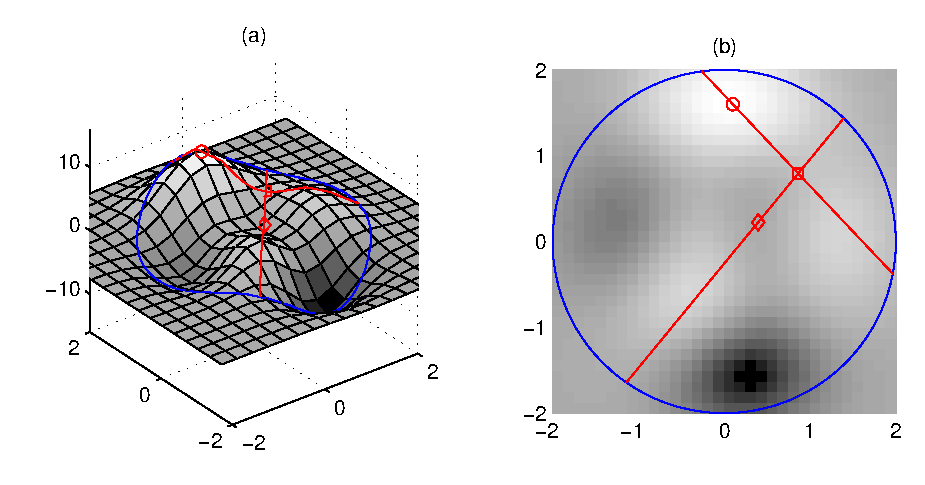
\includegraphics{figures/descent.eps}
\caption{Schematic representation of gradient descent.  Points within the blue
circle are in \calF, the height of the surface the value of
(\ref{eqn:theory:cost function}) at that point.  (a) is a 3D view, (b)
is top view. Red lines show line searches; markers minimums.  Descent
from $\circ$ to $\Box$ to $\Diamond$, where it terminates due to
local minimum.}
\label{fig:gradient descent}
\end{center}
\end{figure}






% commands.tex
% Jeremy Barnes, 1999
% $Id$

\providecommand{\emp}{\mathrm{emp}}
\providecommand{\calF}{\ensuremath{\mathcal{F}}}
\providecommand{\fat}{\ensuremath{\mathrm{fat}}}
\providecommand{\sign}{\ensuremath{\mathrm{sign}}}
\providecommand{\cop}{\ensuremath{\mathrm{co}_p}}
\providecommand{\co}{\ensuremath{\mathrm{co}}}
\providecommand{\bfx}{\ensuremath{\mathbf{x}}}
\providecommand{\bfy}{\ensuremath{\mathbf{y}}}
\providecommand{\bfyh}{\ensuremath{\hat{\mathbf{y}}}}
\providecommand{\calO}{\ensuremath{\mathcal{O}}}
\providecommand{\calI}{\ensuremath{\mathcal{I}}}
\providecommand{\calH}{\ensuremath{\mathcal{H}}}
\providecommand{\calX}{\ensuremath{\mathcal{X}}}
\providecommand{\ip}[2]{\ensuremath{\langle {#1} , {#2} \rangle}}
\providecommand{\lin}{\mathrm{lin}}
\providecommand{\calS}{\ensuremath{\mathcal{S}}}
\providecommand{\VCdim}{\mathrm{VCdim}}
\providecommand{\Fat}[1]{\mathrm{Fat}_{#1}}
\providecommand{\cover}[2]{\mathcal{N}({#1}, {#2})}
\providecommand{\covert}[3]{\mathcal{N}({#1}, {#2}, {#3})}
\providecommand{\MATLAB}{{\tt MATLAB}}
\providecommand{\C}{{\tt C}}
\providecommand{\argmin}{\mathrm{argmin}}

% Theorem-like constructs
\newtheorem{theorem}{Theorem}
\newtheorem{definition}{Definition}

\providecommand{\proof}{\par \par \noindent {\bf Proof:\ }}

\providecommand{\figlinewidth}{1pt}

\newenvironment{linefigure}%
		{\begin{figure} \rule{\textwidth}{\figlinewidth}}%
		{\rule{\textwidth}{\figlinewidth}\end{figure}}


\chapter{Development of algorithms}

\section{Scale invariance}

The boosting algorithm is sensitive only to the relative magnitude of
the classifier weights $b_i$, not to the absolute magnitude.

To see this, consider the linear combination of weights
%
\begin{equation}
y = \sign(F(\bfx)) = \sign(b_1 f_1(\bfx) + b_2 f_2(\bfx) + \cdots +
b_T f_T(\bfx)
\end{equation}
%
Now as
%
\begin{equation}
\sign(\alpha x) = \sign(x) \qquad \qquad \mbox{for $\alpha \neq 0$}
\end{equation}
%
a linear combination that is scaled by an $\alpha \neq 0$
%
\begin{equation}
y = \sign(F(\bfx)) = \sign(\alpha b_1 f_1(\bfx) + \alpha b_2 f_2(\bfx)
+ \cdots + \alpha b_T f_T(\bfx)
\end{equation}
%
is exactly the same as before.

For this reason, normalising of the weight vector is unnecessary.  It
also means that normalising to \emph{any} norm is equivalent to any
other norm; in particular, we will get equivalent behaviour by
normalising in a $p$-norm as we will in a $1$-norm.

\section{Refinement of gradient descent}

Once we have chosen $f_{t+1}$, we need to choose $w_{t+1}$.  This is
chosen to minimise the cost functional along the line given by the
direction $f_{t+1}$.  We can write the value of this cost functional
as
%
\begin{equation}
C = \sum_{i=1}^{m} c \left( y_i F_t(\bfx_i) + y_i w_{t+1}
f_{t+1}(\bfx_i) \right)
\end{equation}
Substituting in $c(f(x)) = e^{-yf(x)}$, we obtain
%
\begin{equation}
C = \sum_{i=1}^{m} \exp \left\{ y_i F_t(\bfx_i) + y_i w_{t+1}
f_{t+1}(\bfx_i) \right\}
\end{equation}
%
Now we need to differentiate this expression with respect to
$w_{t+1}$.   This task is simplified considerably by noting that only
the second half of the exponential term is variable with $w_{t+1}$.
The result is that
%
\begin{eqnarray}{ll}
\frac{\partial C}{\partial w_{t+1}} &
= & \sum_{i=1}^{m} \frac{\partial}{\partial w_{t+1}}
\exp \left\{ y_i F_t(\bfx_i) + y_i w_{t+1}
f_{t+1}(\bfx_i) \right\} \nonumber \\
& = & \sum_{i=1}^{m} y_i \exp \left\{ y_i F_t(\bfx_i) + y_i w_{t+1}
f_{t+1}(\bfx_i) \right\} 
\end{eqnarray}






\chapter{Testing}



\chapter{Discussion}


% conclusion.tex
% Jeremy Barnes, 6/10/1999
% $Id$

\chapter{Conclusion}
\label{chapter:conclusion}

This thesis has considered variants of the AdaBoost machine learning
algorithm, with the desirable property of explicit capacity control,
implemented by confining the combined hypotheses to a $p$-convex hull
of underlying hypotheses.  Theoretical results indicate that these
algorithms should outperform AdaBoost on noisy datasets.

Several ``$p$-boosting'' algorithms were developed: a na\"{\i}ve
approach (which showed no noticeable improvement over AdaBoost), a
``strict'' algorithm confined strictly to the $p$-convex hull at all
times, and a ``sloppy'' variant less restricted during the line
search.

The strict algorithm showed a small improvement over AdaBoost over the
difficult \ds{acacia} dataset, but in general performed poorly
(particularly for $p < 1$).  The poor performance was caused by the
cost functional proving to be strictly increasing, or to have a
minimum very close to the previous hypothesis (in effect the gradient
descent algorithm did not move significantly from its starting point).
Analysis of the features of the cost functional showed that ``easy''
samples produced hill-shaped sample cost functions that would
contribute to a strictly a increasing cost functional.

The sloppy algorithm performed well on noisy datasets, with the shape
of the capacity-vs-gener\-alis\-ation error curve matching the theoretical
prediction, and the generalisation error at the optimal
$p$ value significantly (up to 25\%) improved on AdaBoost (which
already performs \emph{very} well).  While it appears that this
algorithm did find a good solution, which was sparse as predicted by
the theory, it did so in a very inefficient manner (particularly for
$p < 1.2$), with up to several thousand iterations spent adding
hypotheses with weights several hundred orders of magnitude below a
significant level.  A form of the cost function designed to
accelerate the training process is proposed as a potential solution;
alternatively a different optimisation strategy could be used.

It can be concluded that the \emph{concept} of using a $p$-convex hull
has merit as a method of increasing the noise-tolerance of the already
very strong AdaBoost algorithm, but the algorithms that were developed
to \emph{implement} the idea were lacking.

No quantitative comparisons between $p$-boosting algorithms and
other AdaBoost derivatives with similar goals (soft margins
\cite{Ratsch98}, DOOM I/II \cite{Mason99, Mason99a}) were made.
However, these approaches do not appear incompatible with the $p$-convex
hull approach; it is likely that a combined approach would be superior
to both.



\appendix


% Put it back to normal for the non-body parts of the thesis.
\renewcommand{\baselinestretch}{1.0}


\chapter{Acronyms}

Table \ref{tbl:acronyms} is included to benefit the reader who may
get lost in the acronyms that are an inevitable part this thesis.

\begin{table}
\begin{tabular}{l l l}

\bf{Acronym} & \bf{Meaning} & \bf{First introduced} \\ \hline \hline

SLT	& Statistical Learning Theory 	& section \ref{acr:slt} \\
ERM	& Empirical Risk Minimisation 	& section \ref{acr:erm} \\
SRM	& Structural Risk Mininmisation & section \ref{acr:srm} \\
VC dimension & Vapnik-Chervonenkis dimension & section \ref{acr:vcdim} \\
CART	& Classification And Regression Trees & section \ref{acr:cart} \\
\hline

\end{tabular}
\caption{Acronyms}
\label{tbl:acronyms}
\end{table}



% notation.tex
% Jeremy Barnes, 1999
% $Id$

\chapter{Notation and Acronyms}

\newcommand{\notationskip}{5mm}
\newcommand{\notspace}{\vspace{\notationskip}}

\section*{Notation}
\newcommand{\longexp}[1]{\parbox[t]{3in}{\raggedright #1}}
\begin{tabular}{l l c}
\bf{Symbols}		& \bf{Meaning}		& \bf{Section} \\
\hline \hline
$\bfx \in \calI$	& Sample
			& fig \ref{fig:supervised learning} \\

$y \in \calO$		& Label
			& " \\

$X = ((\bfx_1, y_1), \ldots))$
			& Labeled samples, length $m$ (training dataset)
			& \ref{sec:formulation} \\

\notspace
$\calI, \calO$		& Domain and range (usually $\{\pm 1\}$) of problem
			& \ref{sec:domain and range} \\
$h(\cdot) \in \calH : \calI \mapsto \calO$
			& A hypothesis (classifier)
			& \ref{sec:formulation} \\

$\calH$			& A set of possible hypotheses $h$
			& \ref{representation learning machines} \\

$f(\cdot) \in \calF : \calI \mapsto \bbR$
			& \longexp{A non-thresholded hypothesis; usually 
			  $h(\cdot) = \sign(f(\cdot))$}
			& \ref{sec:margin formulation} \\

$\calF$			& A set of possible hypotheses $f$ 
			  ($\calH = \sign(\calF)$)
			& " \\

\notspace
$\bbW : \calI^m \mapsto (\calI \mapsto \calO)$
 			& Learning machine ($\bbW(X) = h$)
			& " \\
$q = Q(\bfx, y, \hat{y})$
			& Loss function
			& \ref{sec:loss function} \\

$R(h)$			& True risk
			& \ref{sec:true risk} \\

$R_{\emp}(h)$		& Empirical risk
			& \ref{sec:empirical risk} \\

$R_{\emp}^w(h)$		& Weighted empirical risk (training error)
			& \ref{sec:weighted empirical risk} \\

\notspace
$R_{\emp}^{\gamma}(h)$	& Margin risk
			& \ref{sec:margin risk} \\

$\VCdim(\cdot)$		& VC dimension
			& \ref{sec:vcdim} \\

$\covert{\calX}{\epsilon}{d(\cdot, \cdot)}$ &
			\longexp{Covering number at scale $\epsilon$ of $\calX$
			using norm $d$ (usually $d_{\infty}$; assumed if not
			specified)}
			& \ref{sec:covering numbers} \\

$\covert{\calX}{\epsilon}{k}$ &
			\longexp{
			Uniform covering number of $\calX$ at scale $\epsilon$
			over length $k$}
			& " \\

\notspace
$\co_{p}(\calX)$, $\co(\calX)$
			& \longexp{$p$-convex hull of set $\calX$; $p=1$
			 assumed if not specified}
			& \ref{sec:p-convex} \\
$\bbB$, $\trainboost$	& AdaBoost, action of AdaBoost
			& \\
$F(\bfx)$, $H(\bfx)$	& \longexp{Boosting hypothesis, nonthresholded
			\& thresholded, $H(\cdot) = \sign(F(\cdot))$}
			& \\

$b_1, \ldots, b_t$	& AdaBoost classifier weights
			& \\

$w_1|_t, \ldots, w_m|_t$ & AdaBoost sample weights
			& \\

\hline
\end{tabular}
\par\par\noindent
A hat ($\hat{\ \ }$) means ``estimate''.  An asterisk ($\ \ ^{\ast}$) means
``optimal'' in some sense.


\section*{Acronyms}

\begin{tabular}{l l l}

\bf{Acronym} & \bf{Meaning} & \bf{First introduced} \\ \hline \hline

SLT	& Statistical Learning Theory 	& \ref{acr:slt} \\
ERM	& Empirical Risk Minimisation 	& \ref{acr:erm} \\
SRM	& Structural Risk Mininmisation & \ref{acr:srm} \\
VC dimension & Vapnik-Chervonenkis dimension & \ref{acr:vcdim} \\
\hline

\end{tabular}



\chapter{Implementation of learning algorithm}


\chapter{Project proposal}

\begin{center}
{\Large DRAFT Honours Project Proposal:
Capacity Control in Boosting via an Adjustable  b Function
\footnote{This project was originally called, ``Aspects
of Statistical Learning Theory and Support Vector Machines''} \\
Jeremy Barnes \\
Supervisor: Dr Bob Williamson}
\end{center}

\section{Introduction}
The aim of this document is to provide some detail on the scope and
implementation of this honours project.  A brief background on the
project is given; followed by an explicit statement of the expected
outcomes; and a timeline.

\section{Background}
Boosting is a method used to improve the generalisation ability of a
"weak" learning algorithm.  It is implemented by generating many
instances of the algorithm, each trained on different data.  This data
is chosen such that examples which are commonly misclassified are
emphasised.  This forces the learning algorithm to work well with the
difficult data, and have better overall performance.  The output of
the boosting algorithm is a weighted combination of the outputs of the
weak learning algorithms (weighted by their performance).

Adjusting the capacity of a learning algorithm controls the size of
the set of possible generalisations.  It is important to control
capacity to avoid overfitting (fitting the noise rather than the
underlying function).  Although boosting is particularly good at
avoiding overfitting, implementing capacity control can improve the
performance of the boosted algorithm [ref] and avoid eventual
overfitting.

The $b$ function is used within the boosting algorithm.  It is
calculated for each instance of the weak learning algorithm, from the
learning error of the weak learning algorithm (the learning error is
the proportion of samples which are misclassified).  In the case of a
binary classification problem, it has the form
%
\begin{equation}
b_t = \log \frac{\epsilon_t}{1-\epsilon_t} \qquad (0 \leq \epsilon_t
\leq 1)
\end{equation}
%	
where $\epsilon_t$ is the learning error of weak learning algorithm  $t$.

	This function describes the ``worth'' of this instance of the weak
learning algorithm.  A plot is shown in figure 1.

\begin{figure}
\begin{center}
\includegraphics{figures/b_func}
\end{center}
\caption{The $b_t$ function versus error $\epsilon_t$}
\end{figure}
 
Weak learners with a value of $\epsilon_t$ around $1/2$ are worthless,
as random guessing performs just as well.  As $epsilon_t$ moves away
from $1/2$, the algorithms become more useful (and show an increase in
$b_t$ ).  Algorithms that approach $\epsilon_t \rightarrow \pm 1$ are
given a $b_t$  that approaches $\pm \infty$.

This project will investigate modifying the b function to become
\begin{equation}
b^{\prime}_t = \mathrm{sign}(b_t) |b_t|^{1/p}
\end{equation}
The new parameter p allows control over how aggressively weak learners
are penalised.  This should allow capacity control via adjustment of
this parameter.

\section{Outcomes}
The project will be successful if the following outcomes are attained:

\begin{itemize}
\item	Enough experimental evidence is gathered to gain an
	appreciation of the effect of the   parameter on the boosting
	algorithm.

\item	From this evidence, some guiding principles for improving the
	performance of the boosting algo-rithm using the   parameter
	are developed.

\item	Theoretical justification of these results is obtained.
\end{itemize}

In addition to these goals, it is hoped that progress in one or more of the following areas will be made:

\begin{itemize}
\item	Performance of the algorithm in problems with varying amounts
	of noise;

\item	Improved versions on the p-boosting algorithm using knowledge
	gained from the theory;

\item	Improving the computational efficiency of boosting using the
	p-boosting algorithm;

\item	Comparisons between p-boosting and other methods of capacity
	control in boosting;

\item	Extension of the results to include arbitrary classification
	problems;

\item	Extension of the results to include regression problems;

\item	Extension of the results to include other enhancements to the
	boosting algorithm, such as "soft margins" \cite{Ratsch98}.
\end{itemize}

In order to limit the project to a reasonable scope, initially the following constraints will be placed:

\begin{itemize}
\item	Only binary classification problems will be considered.

\item	Small datasets will be used.

\item	Simple weak learning algorithms will be used.
\end{itemize}


\section{Timeline}
This section includes a month-by-month description of what I intend to
complete on the project.  It is given in table \ref{table:timeline} on
page \pageref{table:timeline}.

\begin{table}
\begin{tabular}{r l}
\textbf{Month}		& \textbf{Tasks} \\ \hline \hline
December 1998		& Reading \\ \hline
January 1999		& Reading \\ \hline
February 		& Reading \\ \hline
March			& Writing project proposal \\
			& \textbf{19th Project proposal due} \\
			& Obtaining or writing code for experiments \\ \hline
April			& Writing, debugging code \\
			& 12th Code running, first test results \\
			& Obtaining datasets, running tests, refining
			  code  \\ \hline
May			& Running tests \\
			& Developing and testing hypotheses \\
			& Reading on theory \\
			& \textbf{31st First draft of "background"
			  section of thesis} \\ \hline
June			& Initial attempts at theoretical analysis \\
			& Running tests required for theoretical
			  verification \\
			& Attempting to reach closure on some aspects \\
			& \textbf{Exam period} \\ \hline
July			& Attempting to reach closure on some aspects \\
			& Writing progress report \\
			& \textbf{19th Progress report due} \\
			& Preparing for seminar \\
			& \textbf{26th Seminar} \\ \hline
August			& Final work on theory \\
			& Final experimental results to assist theory \\
			& \textbf{30th Sufficient work done to
			  complete thesis} \\ \hline
September		& Work on spin-off or extension aspects \\
			& Preparing for demonstration \\
			& \textbf{27th All experimental and
			  theoretical results obtained} \\
			& Writing thesis \\ \hline
October			& Writing thesis \\
			& \textbf{7th Draft thesis due} \\
			& Revising thesis \\
			& \textbf{27th Thesis due} \\
			& \textbf{28th Demonstration} \\
\hline
\end{tabular}
\caption{Project timeline}
\label{table:timeline}
\end{table}

\noindent\textbf{Notes:}

\begin{itemize}
\item 	I intend to work on the thesis gradually throughout the year,
	so that I do not need to write it all at the end.

\item	I have allowed 2-3 weeks to work on "extension" aspects of the
	problem that are interesting but not vital to a strong thesis.  It
	would not be a serious problem if none of this work can be included in
	the thesis.  These 2-3 weeks also give me some slack if things are not
	going as planned or if I become burnt out and need a break.
\end{itemize}





\backmatter

\nocite{*}

\bibliography{../Bibliography/biblio}
\bibliographystyle{plain}

\end{document}


